% !TeX spellcheck = en_US
\documentclass[french]{yLectureNote}

\title{Mécanique}
\subtitle{Mécanique du point}
\author{Paulhenry Saux}
\date{\today}
\yLanguage{Français}

\professor{S.Deheuvels}%sebastien.deveuhels.irap.omp.eu

\usepackage{graphicx}%----pour mettre des images
\usepackage[utf8]{inputenc}%---encodage
\usepackage{geometry}%---pour modifier les tailles et mettre a4paper
%\usepackage{awesomebox}%---pour les boites d'exercices, de pbq et de croquis ---d\'esactiv\'e pour les TP de PC
\usepackage{tikz}%---pour deiffner + d\'ependance de chemfig
\usepackage{tkz-tab}
\usepackage{chemfig}%---pour deiffner formules chimiques
\usepackage{chemformula}%---pour les formules chimiques en \'equation : \ch{...}
\usepackage{tabularx}%---pour dimensionner automatiquement les tableaux avec variable X
\usepackage{awesomebox}%---Pour les boites info, danger et autres
\usepackage{menukeys}%---Pour deiffner les touches de Calculatrice
\usepackage{fancyhdr}%---pour les en-t\^ete personnalis\'ees
\usepackage{blindtext}%---pour les liens
\usepackage{hyperref}%---pour les liens (\`a mettre en dernier)
\usepackage{caption}%---pour la francisation de la l\'egende table vers Tableau
\usepackage{pifont}
\usepackage{array}%---pour les tableaux
\usepackage{lipsum}
\usepackage{yFlatTable}
\usepackage{multicol}
\newcommand{\Lim}[1]{\lim\limits_{\substack{#1}}\:}
\renewcommand{\vec}{\overrightarrow}
\newcommand{\norm}[1]{||\vec{#1}||}
\begin{document}

%\titleOne
\setcounter{chapter}{1}
	\chapter{Cinématique, forces, équilibre }
Dans ce cours, on s'intéresse à la mécanique du point matériel. Le système d'étude est assimilé à un point matériel qui posséderait l'ensemble de la masse du système, confondu à son centre de gravité. On suppose le centre de gravité et de masse confondu.

C'est une approximation correcte pour des systèmes dont les dimensions sont très petites devant (< <)  les dimensions de l'espace dans lequel ils évoluent.

Exemple : Mouvement de la Terre autour du Soleil. $R_T = 6400 km$, $R_S = 700 000 km$, $d_{ST} = 150\cdot 10^6$. Ici, $R_T, R_S << d_{ST}$, donc on peut appliquer la simplification

\section{Repérage spatio-temporel}
\subsection{repère temporel}
Revient à se donner une origine des temps, évènement pour lequel t=0.
\begin{theorem}[Hypothèse]
On suppose le temps ``universel''. Le temps mis pour effectuer un mouvement est identique pour le système qui bouge et pour un observateur. Cette hypothèse est correcte tant que la vitesse des objets < < vitesse de la lumière, c'est à dire pour des mouvements dits non relativistes.
\end{theorem}

\subsection{Repère spatial}
En général, le mouvement a lieu dans l'espace à trois dimensions, il faut se donner 3 axes non coplanaires, i.e pas dans le même plan ainsi qu'un point de référence (origine).

Exemple : On se donne un repère cartésien (x,y,z)

\subsection{Référentiel}

C'est un solide par rapport auquel on étudie le mouvement et que l'on considère comme fixe durant le mouvement. Le mouvement dépend du référentiel choisi et in faut toujours le préciser.
\section{Rappel de géométrie vectorielle}
\subsection{base cartésienne et repère cartésien}
L'espace à trois dimensions est un espace vectoriel de dimension 3. On dit que 3 vecteurs de l'espace ($\vec{e_x}, \vec{e_y},\vec{e_z}$) forment une base de l'espace s'ils sont dits indépendants. On ne peut pas en écrire un à partir des 2 autres, i.e ne doivent pas \^etre coplanaires.

Dans ce cas, pour tout vecteur $\vec{u}$ de l'espace, il existe une unique décomposition du type $\vec{u} = a\vec{e_x}+ b\vec{e_y}+c\vec{e_z}$.

Schéma 2.2.1

Le choix des vecteurs est arbitraire mais généralement, on va les choisir
\begin{itemize}
 \item orthogonaux entre deux à deux
 \item unitaires (de norme 1)
 \item orientés dans le sens direct (règle ``de la main droite'' : pouce = $\vec{e_x}$, index = $\vec{e_y}$ et majeur = $\vec{e_z}$. Elle est directe si $\vec{e_z} = \vec{e_y} \wedge \vec{e_y}$
\end{itemize}

Si ces 3 conditions sont vérifiées, on dit que la base $B(\vec{e_x}, \vec{e_y},\vec{e_z})$ est une base orthonormée directe (BOND)

\begin{theorem}[Définition]
On appelle repère la combinaison d'une base et d'une origine O : $R(O,\vec{e_x}, \vec{e_y},\vec{e_z})$
\end{theorem}
\subsection{Coordonnées et composantes}
Soit M un point de l'espace muni du repère $R(O,\vec{e_x}, \vec{e_y},\vec{e_z})$. $\vec{OM} = a\vec{e_x}+ b\vec{e_y}+c\vec{e_z}$.

Les quantités scalaires $x,y$ et $z$ sont les coordonnées du point $M$ dans le repère $R$. On écrit $M(x,y,z)_R$.

Tout vecteur $\vec{u}$ peut se décomposer comme $\vec{u} = u_x\vec{e_x}+ u_y\vec{e_y}+u_z\vec{e_z}$

Les scalaires $u_x,u_y,u_z$ sont appelées composantes du vecteur $\vec{u}$ dans le repère $R$. On écrit $\vec{u} (u_x,u_y,u_z)_R$.

Exercice 2.2.2

\subsection{Produit scalaire et norme}
\subsubsection{Norme}
Si la base $B$ est une base orthonormée directe, alors $||\vec{u}|| = \sqrt{u_x^2+u_y^2+u_z^2}$.
\subsubsection{Produit scalaire entre 2 vecteurs}

Schéma 2.2.3

\begin{theorem}[Définition]
$\vec{u}\cdot\vec{v} = ||\vec{u}||\times||\vec{v}|| \times \cos(\theta)$.
\end{theorem}
Proriétés du produit scalaire:

\begin{itemize}
 \item C'est un nombre
 \item $\vec{u}\cdot\vec{u} = ||\vec{u}||^2$
 \item $ \vec{u} \perp  \vec{v} = 0$
 \item Il est commutatif : $\vec{u}\cdot\vec{u} = \vec{v}\cdot\vec{u}$ car $\cos(\theta) = \cos(-\theta)$.
 \item Il est bilinéaire : $(\lambda \vec{u}+\beta \vec{v})\cot \vec{w} = \lambda \vec{u}\cdot \vec{w} + \beta \vec{v}\cdot \vec{w}$.
 \item Dans une BOND, on a $\vec{e_i}\cdot\vec{e_j} = \delta_{ij} (= 0 \iff i\neq j \vee = 1 \iff i=j)$.
 \item Dans une BOND : $\vec{u}\cdot\vec{u} = u_xv_x + u_yv_z+u_zv_z$
\end{itemize}
\subsection{Projection sur une base}
\subsubsection{Méthode 1}

Soit un vecteur $\vec{u} = u_x\vec{e_x}+ u_y\vec{e_y}+u_z\vec{e_z}$. On peut retrouver les composantes du vecteur en effectuant le produit scalaire entre ce vecteur et les vecteurs de la base.

$\vec{u}\cdot\vec{e_x} =  u_x$. De m\^eme, $\vec{u}\cdot\vec{e_y} =  u_y$ et $\vec{u}\cdot\vec{e_z} =  u_z$. On peut donc écrire $\vec{u} = (\vec{u}\cdot\vec{e_x})\cdot \vec{e_x} + (\vec{u}\cdot\vec{e_y})\cdot \vec{e_y} + (\vec{u}\cdot\vec{e_z})\cdot \vec{e_z}$.

\checkInfo{Exemple en 2D}{

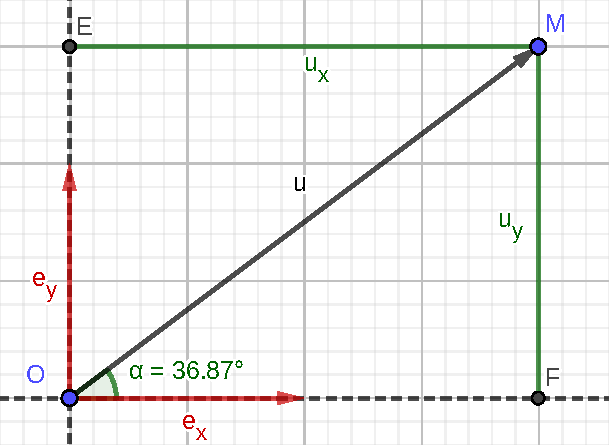
\includegraphics[scale=0.5]{TD2-fig1}

$u_x = \vec{u}\cdot \vec{e_x} = \norm{u}||\vec{e_x}||\cos\theta = ||\vec{u}||\cos\theta$

$u_y = \vec{u}\cdot \vec{e_y} = ||\vec{u}||||\vec{e_y}||\cos(\frac{\pi}{2}- \theta) = ||\vec{u}||\sin(\theta)$}
\criticalInfo{Produit scalaire avec les coordonnées}{}
\subsubsection{Méthode 2}
Projeter $\vec{u}$ dans la base revient à écrire $\vec{u}$ sous la forme $\vec{u} = u_x\vec{e_x}+ u_y\vec{e_y}$ et déterminer $u_x,u_y$. On se place dans un triangle rectangle du schéma précédant

On utilise les relations de trigonométrie : $u_x = ||\vec{u}||\cos(\theta)$ et $u_y = ||\vec{u}||\sin(\theta)$
\subsection{Produit vectoriel}
Soit 2 vecteurs $\vec{u}$ et $\vec{v}$. Le produit vectoriel de $\vec{u}$ et $\vec{v}$, noté $\vec{u} \wedge \vec{v} = \vec{w}$ est l'unique vecteur tel que :

$\vec{w} \perp \vec{u}$ et $\vec{w} \perp \vec{v}$

de norme $\norm{w} = \norm{u} \times \norm{v} \times |\sin(\theta)|$ avec $\theta$ l'angle entre $\vec{u}$ et $\vec{v}$.

De plus, l'ensemble $(\vec{u},\vec{v},\vec{w})$ est une base directe.

$\vec{w}$ est unique car on a défini sa direction, sa norme et son sens.
\subsubsection{Propriétés}
\begin{itemize}
 \item C'est un vecteur
 \item Il est antisymétrique : $\vec{u} \wedge \vec{v} = - \vec{v} \wedge \vec{u}$
 \item Il est linéaire : $(\lambda\vec{u}+\beta\vec{v}) \wedge \vec{w} = \lambda  \vec{u} \wedge \vec{w} + \beta \vec{u} \wedge \vec{w}$
 \item Si $\vec{u}$ et $\vec{v}$ sont colinéaires, $\vec{u} \wedge \vec{v} = \vec{0}$
 \item Si $\vec{u}$ et $\vec{v}$ sont orthogonaux, la norme de $\vec{w}$ est le produit des normes des 2 vecteurs.
 \item Dans une BOND, $\vec{e_x} \wedge \vec{e_y} = \vec{e_z}$ et $\vec{e_x} \wedge \vec{e_z} = -\vec{e_y}$
 \item $||\vec{u}\wedge\vec{v}||$ = aire du parallélogramme engendré par $\vec{u}$ et $\vec{v}$
\end{itemize}
\tipsInfo{Sur le sens du produit dans une BOND}{Quand on le fait de gauche à droite, le produit est positif, dans le cas contraire, il est négatif.}
\subsubsection{Avec les coordonnées}
$\vec{u} = u_x\vec{e_x} +  u_y\vec{e_y} +  u_z\vec{e_z}$

$\vec{v} = v_x\vec{e_x} +  v_y\vec{e_y} +  v_z\vec{e_z}$


Le produit vaut $\vec{u}\wedge \vec{v}=\begin{pmatrix}
u_yv_z-u_zv_y\\
u_zv_x-u_xv_z\\
u_xv_y-u_yv_x
\end{pmatrix}$

\checkInfo{Méthode du Gamma}{
    On écrit côte à côte les deux vecteurs ${\displaystyle {\vec {u}}}$ et ${\displaystyle {\vec {v}}}$ dont on veut faire le produit vectoriel.

    On réécrit $u_x$ en-dessous de $u_z$ et $v_x$ en-dessous de $v_z$

	Pour avoir les coordonnée $x$, on cache les coordonnées suivant x et on fait le ``calcul en ${\displaystyle \gamma }$.

    Pour obtenir les autres coordonnées, on procède de la même manière.

    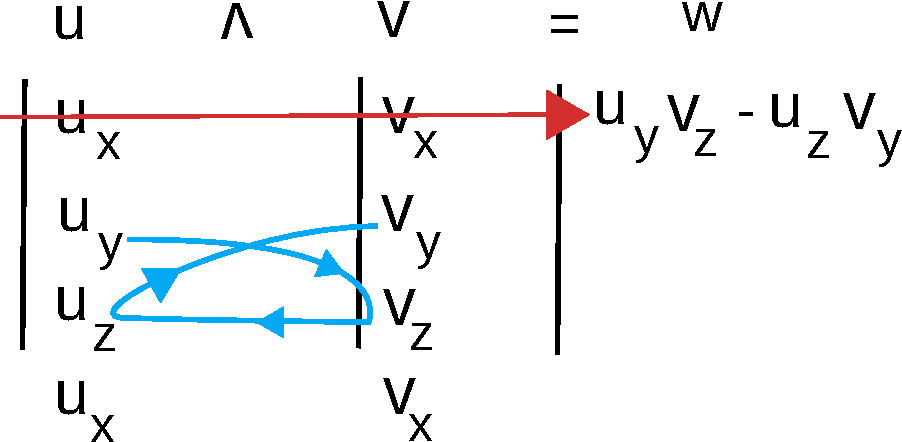
\includegraphics[scale=0.2]{pv1}
    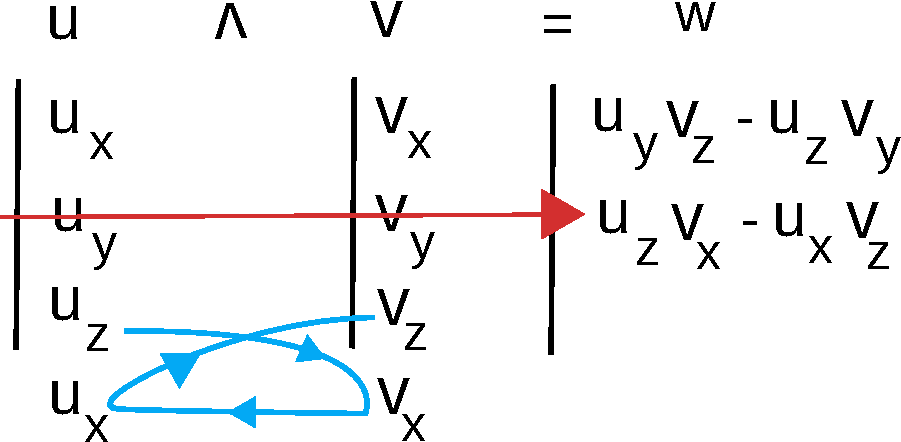
\includegraphics[scale=0.2]{pv2}
    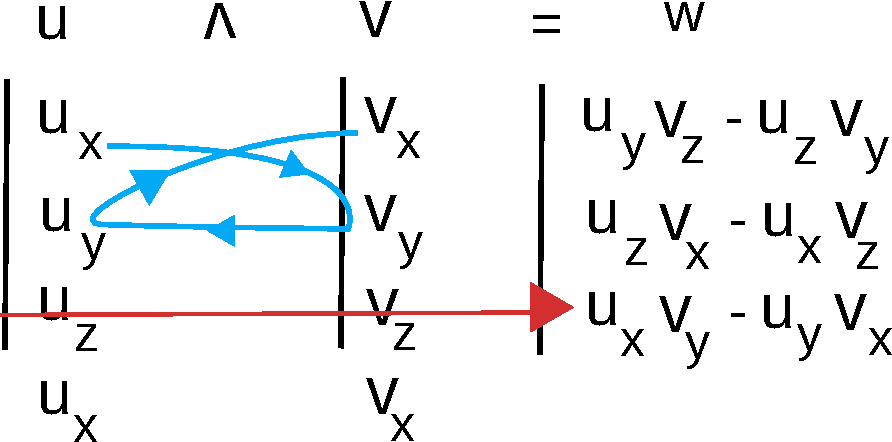
\includegraphics[scale=0.2]{pv3}
    }

\begin{theorem}[Démonstration]
\begin{flalign*}
\vec{u} \wedge \vec{v} &= \left(u_1\, \vec{e}_1 + u_2\, \vec{e}_2 + u_3\, \vec{e}_3 \right) \wedge \left( v_1\, \vec{e}_1 + v_2\, \vec{e}_2 + v_3\, \vec{e}_3 \right)\\
&= u_1\, v_2 \left( \vec{e}_1 \wedge \vec{e}_2 \right) + u_1\, v_3 \left( \vec{e}_1 \wedge \vec{e}_3 \right) + u_2\, v_1 \left( \vec{e}_2 \wedge \vec{e}_1 \right) + u_2\, v_3 \left( \vec{e}_2 \wedge \vec{e}_3 \right)+\dots\\
&= \left( u_1\, v_2 - u_2\, v_1 \right) \left( \vec{e}_1 \wedge \vec{e}_2 \right) + \left( u_2\, v_3 - u_3\, v_2 \right) \left( \vec{e}_2 \wedge \vec{e}_3 \right) \left( u_3\, v_1 - u_1\, v_3 \right) \left( \vec{e}_3 \wedge \vec{e}_1 \right)\\
&= \left( u_1\, v_2 - u_2\, v_1 \right) \vec{e}_3 + \left( u_2\, v_3 - u_3\, v_2 \right) \vec{e}_1 + \left( u_3\, v_1 - u_1\, v_3 \right) \vec{e}_2\\
&= \left( u_2\, v_3 - u_3\, v_2 \right) \vec{e}_1 + \left( u_3\, v_1 - u_1\, v_3 \right) \vec{e}_2 + \left( u_1\, v_2 - u_2\, v_1 \right) \vec{e}_3
\end{flalign*}
\end{theorem}

\section{Cinématique}
C'est l'étude du mouvement sans ses causes.
\subsection{vecteur position}
Soit un point M de l'espace repéré par rapport à un repère R composée d'une BOND. Il représente la position du centre de masse de l'objet. Il dépend du temps car la position de M varie au cours du temps.

Le vecteur $\vec{OM(t)} = x_m(t)\vec{e_x} + y_m(t)\vec{e_y} + z_m(t)\vec{e_z}$

Les quantités $x_m(t), y_m(t) et z_m(t)$ sont les équations horaire du mouvement. Ce sont des équations paramétriques qui indiquent quel mouvement va suivre $M$. On peut en déduire l'équation cartésienne de la trajectoire en supprimant la dépendance au temps

\subsection{Vecteur vitesse}

Le vecteur vitesse du point M par rapport au repère R s'écrit :
\[\vec{v_{M/R}} =  \frac{d\vec{OM(t)}}{dt} = \frac{\vec{OM(t+dt)} - \vec{OM(t)}}{dt}\]
\warningInfo{Direction du vecteur vitesse}{Le vecteur vitesse est toujours tangent à la trajectoire et dans le sens du mouvement}
\subsubsection{Composantes du vecteur vitesse}

\begin{flalign*}
\vec{v_{M/R}} &=  \frac{d\vec{OM(t)}}{dt}\\
&= \frac{d}{dt}(x_m(t)\vec{e_x} + y_m(t)\vec{e_y} + z_m(t)\vec{e_z})\\
&= \frac{d}{dt}(x_m(t)\vec{e_x}) + \frac{d}{dt}(y_m(t)\vec{e_y}) + \frac{d}{dt}(z_m(t)\vec{e_z})\\
&= \dot{x}_m(t)\vec{e_x} + \dot{y}_m(t)\vec{e_y} + \dot{z}_m(t)\vec{e_z}
\end{flalign*}
\subsection{Vecteur accélération}
\begin{flalign*}
\vec{a_{M/R}} &=  \frac{d\vec{v(t)}}{dt}\\
&= \frac{d^2\vec{OM(t)}}{dt^2}
\end{flalign*}
\warningInfo{Direction du vecteur accélération}{Dans le cas général, il n'est pas tangent à la trajectoire.}

\subsubsection{Composantes du vecteur accélération}
\begin{flalign*}
\vec{a_{M/R}} &=  \frac{d\vec{v(t)}}{dt}\\
&= \frac{d}{dt}(v_x(t)\vec{e_x} + v_z(t)\vec{e_y} + v_z(t)\vec{e_z})\\
&= \frac{d}{dt}(v_x(t)\vec{e_x}) + \frac{d}{dt}(v_y(t)\vec{e_y}) + \frac{d}{dt}(v_z(t)\vec{e_z})\\
&= \ddot{x}_m(t)\vec{e_x} + \ddot{y}_m(t)\vec{e_y} + \ddot{z}_m(t)\vec{e_z}
\end{flalign*}
\subsection{Changement de référentiel dans le cas d'une translation}
Soit 2 référentiels R et R' tels que R' est une translation rectiligne par rapport à R avec une vitesse $\vec{V_{R'/R}}$

Dans ce cas on a $\vec{V_{M/R}} = \vec{V_{M/R'}} + \vec{V_{R/R'}}$. C'est la loi de composition des vitesses.

\checkInfo{Exemple du marcheur et nageur}{

R est le référentiel lié au sol et R' lié à l'eau.

On a : $\vec{V_{R'/R}} = V\vec{e_x}$ avec $V=1$m/s.

$\norm{V_{M/R}} = 2$m/s (Vitesse du marcheur par rapport au sol)


$\norm{V_{N/R}} = 2$ (Vitesse du nageur par rapport au à l'eau)


Donc pour le marcheur : $t_A = t_B = \frac{d_{ab}}{\norm{V_{M/R}}} = \frac{6}{2}$

Donc pour le nageur :

Aller : $\vec{V_{N/R}} = \vec{V_{N/R'}} + \vec{V_{R'/R}} = 2\vec{e_x} + \vec{e_x} = 3\vec{e_x}$ donc 3m/s

Retour : $\vec{V_{N/R}} = \vec{V_{N/R'}} + \vec{V_{R'/R}} = -2\vec{e_x} + \vec{e_x} = -\vec{e_x}$ donc 1m/s
}

\subsection{Types de mouvements}
\subsubsection{Mouvement rectiligne}
1 seule dimension
$\vec{a} = a_x\vec{e_x}$

$\vec{v} = v_x\vec{e_x}$

$\vec{OM} = x(t)\vec{e_x}$

\subsubsection{Mouvement uniforme}
Mouvement pour lequel $\norm{V_{M/R}}$ est constant.

\warningInfo{Implications fausse}{Ne veut pas dire que le vecteur vitesse est constant ou que le vecteur accélération est nul (voir orbite de la terre dans le repère de Frenet)}

On a un mouvement uniforme si $\vec{v}\cdot \vec{a} = 0$, donc que $\vec{a}\perp\vec{a}$.

\tipsInfo{Démonstration}{

Le mouvement uniforme $\iff \norm{V_{M/R}}$ = constant

\begin{flalign*}
&\iff \frac{d}{dt} \norm{V_{M/R}} = 0\\
&\iff \frac{d}{dt} \norm{V_{M/R}}^2 = 0\\
&\iff \frac{d}{dt} \vec{V_{M/R}}\cdot\vec{V_{M/R}} = 0\\
&\iff \frac{d\vec{V_{M/R}}}{dt} \cdot \vec{V_{M/R}} + \vec{V_{M/R}}\cdot \frac{d\vec{V_{M/R}}}{dt} = 0\\
&\iff 2 \vec{V_{M/R}}\cdot \vec{a_{M/R}} = 0\\
&\iff \vec{V_{M/R}}\cdot \vec{a_{M/R}} = 0
\end{flalign*}


}

Conséquences :

Si $\vec{v}\cdot\vec{a} > 0$ alors $\frac{d\norm{V_{M/R}}}{dt} > 0$ et $\norm{V_{M/R}}$ augmente au cours du temps (mouvement accéléré).

Si $\vec{v}\cdot\vec{a} < 0$ alors $\frac{d\norm{V_{M/R}}}{dt} < 0$ et $\norm{V_{M/R}}$ diminue au cours du temps (mouvement décéléré).

$\vec{v}\cdot\vec{a} > 0$ si $\cos \alpha > 0 \iff \alpha \in [-\frac{\pi}{2},\frac{\pi}{2}]$.

$\vec{v}\cdot\vec{a} < 0$ si $\cos \alpha < 0 \iff \alpha \in [\frac{\pi}{2},\frac{3\pi}{2}]$.
\section{Rappels sur les lois de Newton}

On fait maintenant de la dynamique, qui consiste à étudier le mouvement à partir de ses causes.
\subsection{Rappel sur le centre de gravité}
Chaque système est considéré comme un point confondu avec son centre de gravité $G$, position définie par le barycentre du système :
\begin{theorem}[Définition du barycentre]
$\displaystyle \sum_i m_i\vec{GM_i} = 0$
\end{theorem}
\subsection{Référentiel galiléen}
C'est un référentiel dans lequel un système isolé (pas de forces) ou pseudo-isolé (résultante des forces nulle) est au repos ou en mouvement rectiligne uniforme (principe d'inertie). C'est un idéal vers lequel on peut tendre mais qu'on atteint pas.

Un référentiel qui en translation rectiligne uniforme par rapport à un référentiel galiléen est aussi galiléen.
\checkInfo{Exemple}{ Le référentiel terrestre (référentiel du laboratoire) : En fait, il est en rotation par rapport à l'axe de rotation de la Terre. Mais il peut \^etre considéré comme galiléen si le temps du mouvement est très petit par rapport à un jour.}
\subsubsection{Référentiel géocentrique}
L'origine est le centre de la Terre avec les axes pointés vers des étoiles lointaines ($\simeq$ fixe) mais il est en rotation autour du Soleil, donc considéré comme galiléen si le temps du mouvement est petit par rapport à une année.
\subsubsection{Référentiel de Copernic}
L'origine est le centre de gravité du système solaire mais aussi en rotation autour du centre de la galaxie $250\cdot10^6$ans.
\subsection{Lois de Newton}
\subsubsection{Principe d'inertie}
Il existe un certain type de référentiels, dits galiléens, dans lesquels ces principes s'appliquent.
\subsubsection{Principe fondamental de la dynamique}
Il s'exprime à partir de la quantité de mouvement $\vec{p_{M/R}} = m\vec{v}$ :

\begin{theorem}[Relation]
\[\frac{d\vec{p_{M/R}}}{dt} = \sum_i \vec{F_i}\]
\end{theorem}

Dans la pratique, la masse du système est souvent constante, dans ce cas :

\begin{theorem}[Relation]
\[\frac{d\vec{p_{M/R}}}{dt} = m\frac{d\vec{v_{M/R}}}{dt} =  m\vec{a} = \sum_i \vec{F_i}\]
\end{theorem}
\subsubsection{Principe d'action réciproque}
La force exercée par A sur B vaut l'opposée de la force exercée par B sur A : $\vec{F_{A/B}} = - \vec{F_{B/A}}$.
\subsection{Exemples de forces}
\subsubsection{Force gravitationnelle}
C'est la première intéraction fondamentale

Soit 2 corps de masse $m_A$ et $m_B$. On a :
\[\vec{F_{g,A/B}} = -G\frac{m_Am_B}{d^2} \vec{e_r}\]

Proriétés :
\begin{itemize}
 \item $\norm{F_g} \simeq \frac{1}{r^2}$.
 \item Elle a une porté infinie
 \item Elle est toujours attractive
 \item Dans le cas particulier du poids, $\vec{F_{g,A/B}} = -m_A \times g$, avec $g = \frac{GM_T}{R_T^2}$. Utiliser le poids n'est pas pénalisé si on est sur/proche de la surface de la Terre. (Pour un satellite, on utilise la force gravitationnelle au lieu du poids).
\end{itemize}
\checkInfo{Remarque}{Dans le contexte de la relativité générale, le concept de force gravitationnelle est remplacé par une courbure de l'espace-temps produite par des objets massifs. }
\subsubsection{Force électrostatique ou force de Coulomb}

Soit 2 charges $q_A$ et $q_B$, distante de $r$. On a, avec $\epsilon_0$ la permittivité du vide :
\[\vec{F_{e,A/B}} = k_e\frac{q_Aq_B}{r^2} \vec{e_r} = \frac{q_Aq_B}{4\pi \epsilon_0r^2} \vec{e_r}\]

Si les 2 charges sont de m\^eme signe, la force est répulsive, dans la cas contraire, elle est attractive.

Elle est analogue à la force gravitationnelle mais elle peut \^etre répulsive.

À l'échelle des particules, cette force domine sur la force gravitationnelle.

\checkInfo{Remarque}{Les 2 autres intéractions fondamentales sont l'intéraction forte (assure la cohésion des noyaux mais a une porté limité <taille des noyaux d'atome) et l'intéraction faible (responsable de la désintégration radioactive)}
\subsubsection{Poussée d'Archimède}

On isole une quantité de fluide. S'il n'y avait que le Poids, il coulerait. or ce n'est pas la cas, il est en repos. Il faut donc une force de m\^eme diretion et norme et de sens opposé. Donc $\vec{\pi} = - \vec{P}$.

\begin{theorem}[Expression de la poussée d'Archimède]
Tout corps plongé dans un fluide (gaz ou liquide) est soumis à une force, appelée poussée d'Archimède qui à la m\^eme direction que le poids, de sens opposé et dont la norme est égale au poids du volume de fluide déplacé.
\end{theorem}
\checkInfo{Exemple}{Exemple 1 : On prend un objet. Voir schéma. $\norm{\pi} = V_i\times \rho_f \times g$.

Exemple 2 : Cas où le corps est complètement immergé : $\norm{\pi} = \rho_fVg$ et $\norm{P} = mg = \rho_0Vg$. On se demande si le corps descent, remonte ou reste sur place.

D'après la seonde loi de newton :

\begin{flalign*}
m\vec{a} &= \sum \vec{F_i}\\
\rho_0Va_z\vec{e_z} &= -\rho_0Vg\vec{e_z}+\rho_fVg\vec{e_z}\\
\rho_0a_z\vec{e_z} &= -\rho_0g\vec{e_z}+\rho_fg\vec{e_z}\\
\rho_0a_z &= -\rho_0g+\rho_fg\\
a_z &= \frac{-\rho_0g+\rho_fg}{\rho_0}\\
a_z &= \frac{-\rho_0g+\rho_fg}{\rho_0}
\end{flalign*}
Ainsi, l'objet flotte si la masse volumique est plus faible que celle de l'eau.
}
Généralement, on néglige la poussée d'archimède dans l'air car $\rho_{air} = 1.2kg/m^3$ à l'expetion des mongolfières.
\criticalInfo{Ordre de grandeur de masse volumique}{
 $\rho_{air} = 1.2kg/m^3$ et $\rho_{eau} = 1000kg/m^3$}
 \subsubsection{Réaction du support}
 Si un support s'oppose à la chute d'un corps, il exerce sur lui une force appelée réaction du support (Exemple d'un objet immobile sur une table où elle est de m\^eme norme et de sens différent).

 En l'absence de frottements solides, la réaction du support est orthogonale au mouvement. Dans le cas contraire, le support s'oppose au mouvement
 \subsection{Équilibre statique}
 Dans un référentiel galiléen, le principe d'inertie s'applique t on a l'équivalence $\sum_i \vec{F_i} = \vec{0} \iff \vec{a} = \vec{0}$. Le système est au repos ou en mouvement rectiligne uniforme
 \checkInfo{Exemple d'application}{Si on sait qu'un objet est à l'équilibre statique, on sait que l'accélération est nulle est donc que la somme des force vaut 0.

 Imaginons une voiture en panne sur une route. On essaye de bouger la voiture, mais elle ne bouge pas}
\subsection{Résolution d'un problème de dynamique}
Exemple de la chute libre (Ex4): Lancer d'un ballon : On se donne un repère R et on va dire que le ballon est initialement à l'origine.
\subsubsection{Définir le système d'étude}
Ici, le sytème est {Ballon}
\subsubsection{Définir un référentiel d'étude et un repère}
Ici, c'est le référentiel terrestre, que l'on consière galiléen, avec un repère $R(0,\vec{e_x},\vec{e_y},\vec{e_z})$.
 \subsubsection{Faire un bilan des forces}
 Ici, uniquement le poids $\vec{P}$ avec les frottements de l'air négligés.
\subsubsection{Appliquer le PDF}
$m\vec{a_{b/r}}  = \sum \vec{F} = \vec{P}$
\subsubsection{Projeter les forces et le vecteur accélération suivant les axes du repère}
Pour cela, il faut déterminer le nombrede dimension du problème et projeter : $\vec{P} = -mg\vec{e_z}$. On a aucun mouvement suivant $y$ car pas de force dans cette direction et pas de vitesse initiale suivant $y$. Donc le mouvement se fait dans le plan $(Oxz)$.

On projette $\vec{a}$. le PDF projeté suivant les axes s'écrit :
$m\begin{pmatrix}
\ddot{x}\\\ddot{y}\\\ddot{z}
\end{pmatrix} = \begin{pmatrix}
0\\0\\-mg
\end{pmatrix}$

On obtient autant d'équations scalaires que de dimensions du problème.
\begin{flalign*}
m\ddot{x} &= 0\\
m\ddot{y} &= 0\\
m\ddot{z} &= 0
\end{flalign*}
\subsubsection{Intégrer une première fois pour obtenir la vitesse}
\begin{flalign*}
\dot{x} &= A\\
\dot{y} &= B\\
\dot{z} &= -gt+C
\end{flalign*}

Donc, en déterminant les constantes
\begin{flalign*}
\dot{x} &= v_0\cos(\alpha)\\
\dot{y} &= 0\\
\dot{z} &= -gt+ v_0\sin(\alpha)
\end{flalign*}
\subsubsection{Intégrer pour obtenir la position}
\begin{flalign*}
\dot{x} &= v_0\cos(\alpha)t+A'\\
\dot{y} &= A\\
\dot{z} &= -gt^2\frac{1}{2}+ v_0\sin(\alpha)t + C
\end{flalign*}
On détermine les conditions initiales et on trouve :
\begin{flalign*}
\dot{x} &= v_0\cos(\alpha)t\\
\dot{y} &= 0\\
\dot{z} &= -gt^2\frac{1}{2}+ v_0\sin(\alpha)t
\end{flalign*}
On obtient ainsi les équations horaire du mouvement
\subsubsection{Calculer l'équation cartésienne de la trajectoire}
Il faut éliminer le temps.

On va utiliser l'équation en $x$ pour trouver que $t=\frac{x}{v_0\cos(\alpha)}$ et l'injecter dans l'expression de $z(x) = -\frac{g}{2v_0^2\cos^2\alpha}x^2 + \tan(\alpha)x$. C'est l'équation d'une parabole.
\subsubsection{Points remarquable}
\begin{itemize}
 \item Altitude maximale : correspond au point où la vitesse verticale s'annule : On veut que $v_z$ au temps $t_1$ soit égale à 0. On utilise l'expression de $v_z = -gt+v_0\sin(\alpha)$ pour trouver le temps où $v_z = 0$. L'altitude maximale vaut $z_{t1}$. On utilise l'équation horaire pour déterminer $z$ en $t_1$.
\end{itemize}
\section{Frottements solides}
\subsection{Approche phénoménologique}
\begin{theorem}[Définition]
Elles sont liée au contact entre 2 surfaces
\end{theorem}
Exemple en l'absence de mouvement : Voir schéma 5.1. Le bilan des forces est $\vec{P},\vec{F},\vec{R}$ et on a : $\vec{P}+\vec{F}+\vec{R} = \vec{0}$ On aura donc nécessairement pour $\vec{R}$
\begin{itemize}
 \item une composante normale $\vec{N}$ qui s'oppose au poids
 \item une composante tangentielle $\vec{T}$ qui s'oppose à $\vec{F}$. Elle correspond aux forces de frottement solide et dépend des matérieux des surfaces en contact
\end{itemize}
Si la norme de $\vec{F}$ augmente, l'objet finit par se mettre en mouvement.

Quand $\norm{F}$ dépasse $\mu_s\vec{N}$, l'objet se met en mouvement. $\mu_s$ est le coefficient de frottement statique, sans dimension.

Quand l'objet est en mouvement, la norme de $\norm{T}$ reste contsnate et vaut $\mu_d\vec{N}$. $\mu_d$ est le coefficient de frottement dynamique, sans dimension. On a toujours $\mu_d<\mu_s$.
\begin{center}
\begin{tabular}{lll}
Matériaux & $\mu_s$ & $\mu_d$\\
acier/acier & 0.74 & 0.57\\
gomme/béton & 1 & 0.8\\
glace/glace & 0.1 & 0.03\\
articulation d'un humain & 0.01 & 0.003
\end{tabular}
\end{center}
\subsection{Lois de Coulomb}
Elles sont empirique, i.e déduites de l'expérience. La réaction du support est décomposée en $\vec{R} = \vec{T}+\vec{N}$
\begin{theorem}[Lois]
\begin{itemize}
 \item Il y a équilibre si $\norm{T} \leq \mu_s \norm{N}$
 \item Si il y a un glissement, $\norm{T} = \mu_d \norm{N}$ et $\vec{T}$ dans la direction opposé au mouvement, c'est à dire : $\vec{T} = -\norm{T}\times \frac{\vec{v}}{\norm{v}}$.
\end{itemize}
\end{theorem}
\subsection{Méthode de résolution}

Pour résoudre un problème avec des frottements solides
\subsubsection{On suppose l'équilibre}
\subsubsection{On écrit le principe fondamental de la statique}
\[\sum \vec{F} = F\vec{F_1}+\dots +\vec{T}+\vec{N} = \vec{0}\]
Les normes de T et N sont inconnues pour le moment.
\subsubsection{On en déduit les valeurs de T et N}
Soit $\norm{T} \leq \mu_s\norm{N}$, il y a bien équilibre

Soit $\norm{T} > \mu_s\norm{N}$, il y a glissement. On écrit alors le PFD avec $\vec{T} = -\norm{T}\times \frac{\vec{v}}{\norm{v}}$.
\subsection{Exemple du solide sur le plan incliné}
On donne $\mu_s, \mu_d$ le coefficient de frottement statique et dynamique entre le solide et le plan incliné.

\begin{itemize}
 \item Sytème : {Masse $m$}
 \item Référentiel terrestre + repère $R(0,\vec{e_x},\vec{e_y})$.
\end{itemize}
\subsubsection{On suppose l'équilibre}
Dans ce cas, $\sum\vec{F} = \vec{0}$ et $\vec{P}+\vec{T}+\vec{N} = \vec{0}$.

On fait la projectiond des forces dans $R$ :
$\vec{P} = -\norm{P}\sin\alpha \vec{e_x} - \norm{P}\cos\alpha\vec{e_y} = -mg(\sin\alpha \vec{e_x} + \cos\alpha\vec{e_y}) $.

$\vec{T} = T \vec{e_x} + 0 c{e_y} $ avec T positif ou négatif

$\vec{N} = 0 \vec{e_x} + N c{e_y} $ avec N positif ou négatif

On réécrit les équations :
\[\left\{\begin{matrix}
-mg\sin\alpha + T +0 = 0 &\Rightarrow T = mg\sin\alpha\\
-mg\cos\alpha + 0+N = 0 &\Rightarrow N = mg\cos\alpha 0
\end{matrix}\right.
\]

On vérifie si c'est à l'équilibre.

On calcule $\displaystyle \frac{\norm{T}}{\mu_s\norm{N}} = \frac{mg\sin\alpha}{\mu_s mg\cos\alpha} = \frac{\tan\alpha}{\mu_s}$.

On a équilibre si $\displaystyle \norm{T} \leq \mu_s\norm{N} \iff \frac{\tan\alpha}{\mu_s} \leq 1 \iff \mu_s\geq \tan \alpha \iff \alpha \leq \tan^{-1}\mu_s$.

Si $\mu_s< \tan \alpha$, alors l'équilibre n'est pas possible. Il y a glissement et d'après la deuxième Loi de Coulomb, $\norm{T} = \mu_d\norm{N}$ et $\vec{T}$ opposé au mouvement.

\subsubsection{Il y a mouvement}
On écrit le PFD : $\sum\vec{F} = m\vec{a}$. On a donc :

\[\left\{\begin{matrix}
-mg\sin\alpha + T  &= m\ddot{x}\\
-mg\cos\alpha + 0+N &= m\ddot{y}
\end{matrix}\right.
\]
Mais il n'y a pas de mouvement selon $y$ donc, donc $\ddot{y} = 0$. On obtient :
\[\left\{\begin{matrix}
-mg\sin\alpha + T - m\ddot{x} &= 0\\
-mg\cos\alpha + 0+N &= m\times 0
\end{matrix}\right.
\Rightarrow N = mg\cos\alpha
\]

Mais $\norm{T} = \mu_d\norm{N} = \mu_dmg\cos\alpha$, donc $T = \mu_dmg\cos\alpha$.

On peut réécrire l' équation, pour obtenir $\ddot{x}$ :
\begin{flalign*}
&-mg\sin\alpha + T -m\ddot{x} = 0\\
&-mg\sin\alpha + \mu_dmg\cos\alpha -m\ddot{x} = 0\\
&\iff -mg\sin\alpha + \mu_dmg\cos\alpha = m\ddot{x}\\
&\iff -g(m\sin\alpha - \mu_dm\cos\alpha) = m\ddot{x}\\
\end{flalign*}

On obtient donc : $\ddot{x} = -g(\sin\alpha - \mu_d\cos\alpha)$, qui est constante.

\end{document}

